\section{Введение}

\textbf{Цель работы:}
1) прямое измерение кривых нагревания $T_{heat}(t)$ и охлаждения
$T_{cool}(t)$пустого калориметра и системы «калориметр + твердое тело»; 2)
определение коэффициента теплоотдачи стенок калориметра; 3) определение
теплоемкости пустого калориметра и удельной теплоемкости твердого тела

\textbf{В работе используются:}
калориметр с нагревателем и термометром
сопротивления; универсальный вольтметр В7-78/3 в режиме омметра, измеритель
температуры - термопара K-типа совместно с универсальным вольтметром В7-78/2,
источник питания GPS-72303, универсальные вольтметры В7-78/3 (в режиме
амперметра) и KEITHLEY (в режиме вольтметра) для измерения мощности
нагревателя, компьютерная программа АКИП для сопряжения персонального
компьютера и универсальных вольтметров В7-78/2 и В7-78/3.


В данной работе измерение теплоемкости твердых тел производится
по стандартной схеме. Исследуемое тело помещается в калориметр с
нагревателем мощностью $P$. Пусть $\Delta Q$ -- количество тепла, подведенное к
системе «тело + калориметр» за время $\Delta t$, а $\Delta T$ -- изменение её
температуры, произошедшее в результате подвода тепла $\Delta Q$. Тогда
согласно определению теплоемкость системы «тело + калориметр»
будет равна:

\begin{equation}
    C = \frac{\Delta Q}{\Delta T}.
    \label{eq:qDqT}
\end{equation}

Температура внутри калориметра надежно измеряется термометром (в
нашем случае — термометром сопротивления). В реальных условиях $\Delta Q \neq P\Delta t$ , так как часть энергии, выделенной нагревателем, уходит из
калориметра благодаря теплопроводности его стенок. В результате
количества тепла $\Delta Q = C\Delta T$ , подведенное к системе «тело +
калориметр» будет меньше $P\Delta t $ на величину тепловых потерь:
\begin{equation}
    C\Delta T = P\Delta t - \lambda\left(T-T_\text{К}\right)\Delta t,
    \label{eq:C_Delta_T}
\end{equation}
где $\lambda$ -- коэффициент теплоотдачи стенок калориметра, $T$ -- температура
тела и калориметра, $T_\text{К}$ -- температура окружающего калориметр воздуха (комнатная).

Уравнение (\ref{eq:C_Delta_T}) является основной расчетной формулой работы. В дифференциальной форме для процессов нагревания и охлаждения ($P = 0$) соответственно оно имеет следующий вид:
\begin{equation}
    CdT = Pdt - \lambda\left[T_{heat}(t) - T_\text{К}(t)\right]dt,
    \label{eq:CdT}
\end{equation}
\begin{equation}
    Cdt = -\lambda\left[T_{cool}(t) - T_\text{К}(t)\right]dt,
    \label{eq:CdT2}
\end{equation}
где $P$ -- мощность нагревателя, $\lambda$ -- коэффициент теплоотдачи стенок
калориметра, $t$ – время, измеряемое от момента включения нагревателя,
$T_{heat}(t)$ -- температура тела в момент времени $t$ на кривой нагревания,
$T_{cool}(t)$ -- температура тела в момент времени $t$ на кривой охлаждения,
$T_\text{К}(t)$ -- температура окружающего калориметр воздуха (комнатная) в
момент времени $t$, $dt$ -- время, в течение которого температура тела
изменилась на $dT$.

\subsection{Эксперементальная установка}

\begin{figure}[h]
    \centering
    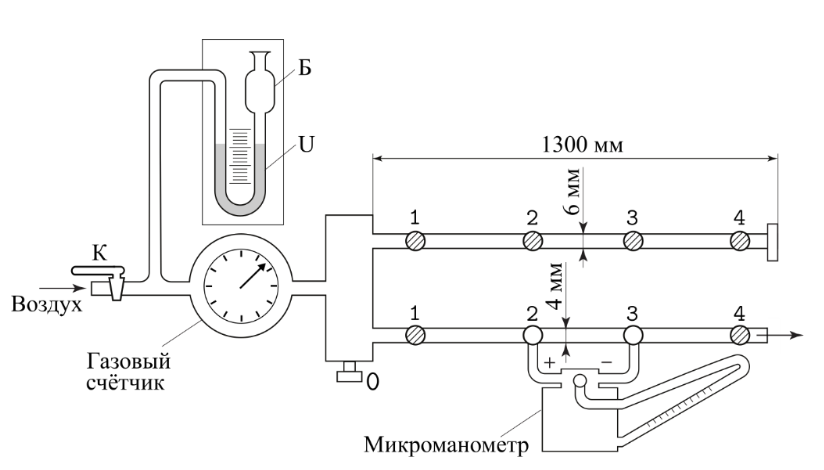
\includegraphics[width = 0.6\linewidth]{ust.png}
\end{figure}

Установка состоит из калориметра с пенопластовой изоляцией,
помещенного в ящике из многослойной клееной фанеры. Внутренние стенки калориметра выполнены из материала с высокой
теплопроводностью. Надежность теплового контакта между телом и
стенками обеспечивается их формой: они имеют вид усеченных конусов
и плотно прилегают друг к другу.

Для выталкивания образца служит винт в донышке внутренней стенки
калориметра. В стенку калориметра вмонтированы спираль нагревателя
(СН) и спираль термометра сопротивления (далее термометр или
терморезистор).

Экспериментально измеряемые данные:
\begin{enumerate}
    \item $R_{heat}(t)$ -- кривая зависимости термометра сопротивления от времени при нагревании калориметра с телом при $P = const$ .
    \item $R_{cool}(t)$ -- кривая зависимости термометра сопротивления от времени при охлаждении калориметра с телом при $P = 0$(нагреватель выключен!).
    \item $T_\text{К}(t)$ -- кривая зависимости комнатной температуры от времени
\end{enumerate}
Кривые $R_{heat}(t)$, $R_{cool}(t)$ и $T_\text{К}(t)$ записываются по точкам c шагом по
оси времени $\Delta t = 1$ с при помощи компьютерной программы АКИП,
напрямую (через USB разъем) связанную с цифровыми вольтметрами
В7-78/2 и В7-78/3, работающими соответственно в режиме измерения
температуры (термопара K-типа) и омметра с подключением по 4-х
проводной схеме.

\subsection{Методика эксперемента}
Температура измеряется термометром сопротивления. Сопротивление проводника изменяется с температурой по закону

\begin{equation}
    R_{T} = R_{273}(1 + \alpha (T - 273)),
    \label{RT}
\end{equation}
где $R_{T}$ -- сопротивление термометра про $T  ^{\circ}C$, $R_{0}$ -- его сопротивление при $0  ^{\circ}C$, $\alpha$ -- температурный коэффициент сопротивления.

Выразим сопротивление $R_{273}$ через измеренное значение $R_{к}$ -- сопротивление термометра при комнатной температуре. Согласно (\ref{RT}), имеем

\begin{equation}
    R_{273} = \frac{R_{к}}{1 + \alpha (T_\text{К} - 273)},
    \label{R273}
\end{equation}

Подставляя (\ref{R273}) в (\ref{RT}), найдём:

\begin{equation}
    T(R_T) = 273 + \frac{R_T}{\alpha R_\text{К}} \left[ 1 + \alpha (T_\text{К} - 273) \right] - \frac{1}{\alpha}
    \label{T_R_T}
\end{equation}

Формула (\ref{T_R_T}) позволяет легко пересчитать кривые $R_{heat}(t)$, $R_{cool}(t)$ в кривые $T_{heat}(t)$, $T_{cool}(t)$. Входящий в формулу температурный коэффициент сопротивления меди равен $\alpha = 4.28*10^{-3} град^{-1}$.

Из уравнения (\ref{eq:CdT2}) при $T_\text{К}(t) = T_\text{К} = const$:

\begin{equation}
    C dT_{cool} = - \lambda \left[ T_{cool} - T_\text{К} \right] dt
    \label{C_dT_cool}
\end{equation}

Это дифференциальное уравнение с разделяющимися переменными $T_{cool}$ и $t$:

\begin{equation}
    \frac{C dT_{cool}}{- \lambda \left[ T_{cool} - T_{к} \right]} = dt
    \label{eq:diff}
\end{equation}

После интегрирования в пределах от $t=0$ ($T_{cool} = T$) до произвольного момента времени $t$:

\begin{equation}
    \frac{-C}{\lambda} ln \frac{T_{cool} - T_\text{К}}{T - T_\text{К}} = t
    \label{eq:diff_integral}
\end{equation}

Отсюда находим явную зависимость от времени:

\begin{equation}
    T_{cool}(t) = (T - T_\text{К}) e^{\frac{- \lambda}{C} t} + T_\text{К}
    \label{T_cool_t}
\end{equation}

Уравнение (\ref{T_cool_t}) легко спрямляется в координатах ($ln \frac{T_{cool} - T_\text{К}}{T - T_\text{К}}$, $t$). Тангенс угла наклона данной прямой позволяет определить отношение искомых величин $\frac{\lambda}{C}$.

Из уравнения (\ref{eq:CdT}) при $T_\text{К}(t) = T_\text{К} = const$:

\begin{equation}
    C dT_{heat} = P dt - \lambda \left[ T_{heat} - T_\text{К} \right] dt
    \label{C_dT_heat}
\end{equation}

Это дифференциальное уравнение с разделяющимися переменными $T_{heat}$ и $t$:

\begin{equation}
    \frac{C dT_{heat}}{P - \lambda \left[ T_{heat} - T_{к} \right]} = dt
    \label{eq:diff2}
\end{equation}

После интегрирования в пределах от $t = 0$ ($T_{heat} = T_\text{К}$) до произвольного момента времени $t$:

\begin{equation}
    \frac{-C}{\lambda} ln \frac{P - \lambda (T_{heat} - T_{к})}{P} = t
    \label{eq:diff_integral2}
\end{equation}

Отсюда находим явную зависимость от времени:

\begin{equation}
    T_{heat}(t) = \frac{P}{\lambda} (1 - e^{\frac{-\lambda}{C} t}) + T_\text{К}
    \label{T_heat_t}
\end{equation}

Уравнение (\ref{T_heat_t}) позволяет по найденному ранее из кривой охлаждения отношению $\frac{\lambda}{C}$ определить $\lambda$, а зная $\lambda$ и $\frac{\lambda}{C}$ легко найти искомую теплоемкость $С$.

Метод измерений величин $С$ и $\lambda$ рассмотренный выше, дает хорошие результаты при стабильной комнатной температуре во время проведения эксперимента и является по своей сути интегральным. $С$ и $\lambda$ определяются из уравнений (\ref{T_cool_t}) и (\ref{T_heat_t}), которые следуют из уравнений (\ref{eq:CdT}) и (\ref{eq:CdT2}) после их интегрирования. При существенных колебаниях комнатной температуры ($\sim 2-3~^0C$) интегральные уравнения (\ref{T_cool_t}) и (\ref{T_heat_t}) могут привести к достаточно большой погрешности в определении величин $С$ и $\lambda$. В этом случае следует использовать дифференциальные методы, основанные на измерении величин $\left( \frac{dT}{dt} \right)_{heat}$ и $\left( \frac{dT}{dt} \right)_{cool}$ в окрестностях каких-либо «удобных» точек. К таким «удобным» точкам относится точка на кривой нагревания, при которой температура калориметра совпадает с комнатной. Действительно, дифференцируя уравнение (\ref{eq:CdT}) по времени при $T_{heat}(t) = T_\text{К}(t)$, получим простую и удобную формулу для определения теплоемкости $С$:

\begin{equation}
    C = \frac{P}{(dT_{heat} / dt)_{T = T_\text{К}}}
    \label{eq:C}
\end{equation}

Она дает хорошие результаты, если ее применение никак не связано с моментом включения нагревателя. Причина проста: сразу после включения нагревателя в калориметре происходят переходные процессы формирования тепловых потоков, которые не описываются уравнением (\ref{eq:CdT}) и соответственно уравнением (\ref{eq:C}). Чтобы обойти данную трудность, перед включением нагревателя необходимо охладить калориметр до температуры на $\sim 2-5~^oC$ ниже комнатной. В этом случае при подходе к точке $T_{heat}(t) = T_\text{К}(t)$ все переходные процессы уже закончатся и уравнение (\ref{eq:C}) будет корректным.

Другими «удобными» точками для определения $С$ и $\lambda$ являются точки при одной и той же температуре $T$ на кривых нагревания $T_{heat}(t)$ и охлаждения $T_{cool}(t)$ соответственно. Действительно продифференцируем уравнения (\ref{eq:CdT}) и (\ref{eq:CdT2}) по времени:

\begin{equation}
    C \left( \frac{dT}{dt} \right)_{heat} = P - \lambda \left[ T_{heat}(t) - T_\text{К}(t) \right]
    \label{eq:C_diff_heat}
\end{equation}
\begin{equation}
    C \left( \frac{dT}{dt} \right)_{cool} = - \lambda \left[ T_{cool}(t) - T_\text{К}(t) \right] \label{eq:C_diff_cool}
\end{equation}

Определим $A = \left( \frac{dT}{dt} \right)_{heat}$ и $B = \left( \frac{dT}{dt} \right)_{cool}$ при одной и той же температуре $T$ на кривых $_{heat}(t)$ и $T_{cool}(t)$ соответственно. Тогда с учетом введенных обозначений, решая систему уравнений (\ref{eq:C_diff_heat}) и (\ref{eq:C_diff_cool}), получим следующие выражения для $С$ и $\lambda$:

\begin{align}
    \lambda &= \frac{P}{(T - T_{к2})(1 - \frac{A}{B}) + T_{к2} - T_{к1}} \label{eq:lambda}\\
    C &= \frac{P}{A - B + A \frac{T_{к1} - T_{к2}}{T - T_{к1}}} \label{eq:C2}
\end{align}
где $T_{к1}$ и $T_{к2}$ -- комнатная температура в моменты времени $t = t_1$ и $t = t_2$, когда $T_{heat}(t_1) = T_{cool}(t_2) = T$.

В случае равенства комнатных температур, когда $T_{\text{К}1} = T_{\text{К}2} = T_\text{К}$ формулы (\ref{eq:lambda}) и (\ref{eq:C2}) упрощаются

\begin{equation}
    \lambda = \frac{P}{(T - T_\text{К})(1 - \frac{A}{B})}
    \label{eq:lambda_fin}
\end{equation}
\begin{equation}
    C = \frac{P}{A - B}
    \label{eq:C_fin}
\end{equation}

\begin{figure}[ht]
    \centering
    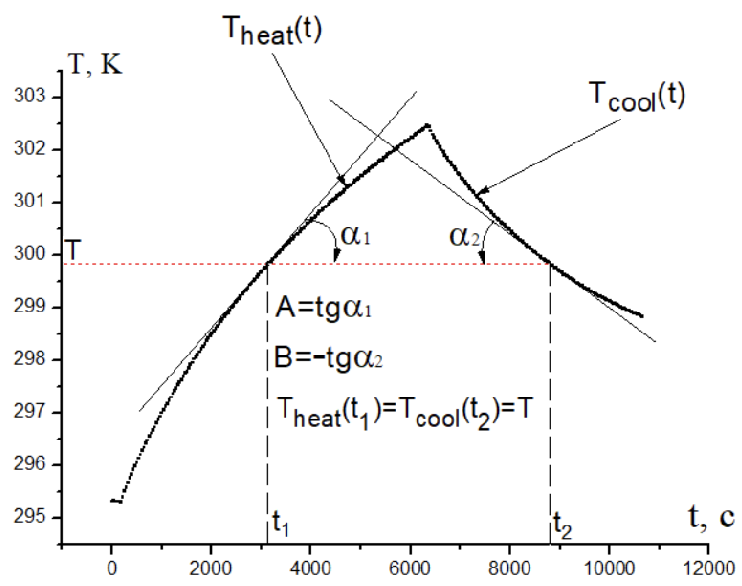
\includegraphics[width=0.5\textwidth]{diff_method.png}
\end{figure}

Следует иметь в виду, что определение величины $B$ на кривой охлаждения $T_{cool}(t)$ необходимо производить на участках кривой достаточно далеких от момента выключения нагревателя, после того как в калориметре закончатся переходные процессы «переполюсовки» тепловых потоков. Корректный интервал времени для определения В можно определить экспериментально из кривой $T_{cool}(t)$, спрямляя ее в координатах ($ln \frac{T_{cool} - T_\text{К}}{T - T_\text{К}}$, $t$) , после чего исключить из рассмотрения начальный нелинейный участок:

\begin{figure}[ht]
    \centering
    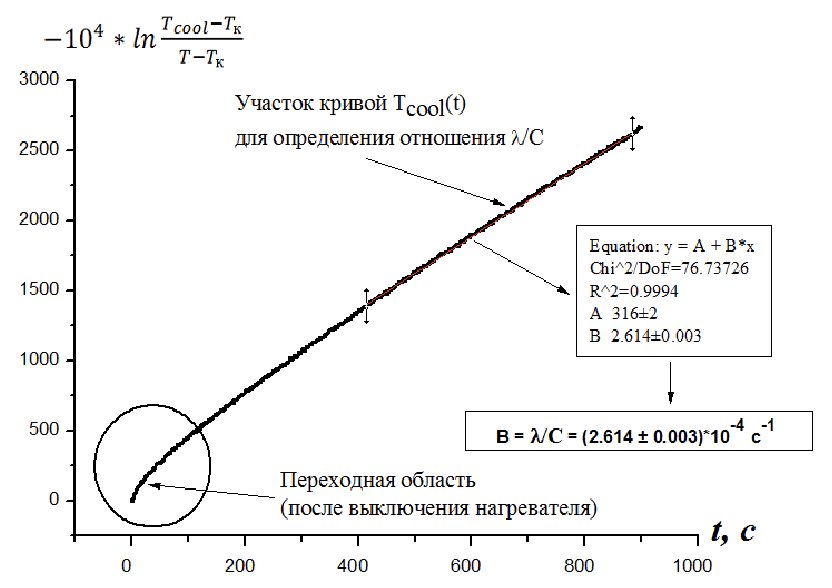
\includegraphics[width=0.5\textwidth]{not_lin_fragment.png}
\end{figure}
